\section{Re-Implementation \& Results}

\begin{frame}
    \frametitle{Re-Implementation Tools}
	\begin{table}
		\centering
		\caption{Comparison Setup \& Tools}
		\label{tab:tools}
		\begin{tabular}{lccccccc}
			\toprule
			& \textbf{Original Paper} & \textbf{Reproduction}\\
			\midrule
			Hardware & Thinkpad L450 & Matebook X Pro (1st Generation)\\
			Operating System & Debian 9 (Stretch) & Ubuntu 20.04\\
			Firefox & 62.0.2 / 61.0.2 & 84.0.2 \\
			Chrome & 69 & 88 \\
			Selenium & 3.14.0 & 3.141.59\\
			Geckodriver & 0.21.0 & 0.29.0\\
			HAR Export Trigger & 0.6.1 & 0.6.1\\
			\bottomrule
		\end{tabular}
	\end{table}
	
Despite trying the versions specified in the original paper as well as the more modern versions, \textbf{it was not possible to consistently extract HAR files using Firefox with Selenium and Chrome with PyDevTools as specified in the original paper}.

$\boldsymbol{\rightarrow}$  This paper focused on reproducing measurements using Firefox with Marionette.
\end{frame}

\begin{frame}
    \frametitle{Results - Redirects}
\begin{figure}
 \centering
 \begin{subfigure}{0.5\textwidth}
 \centering
	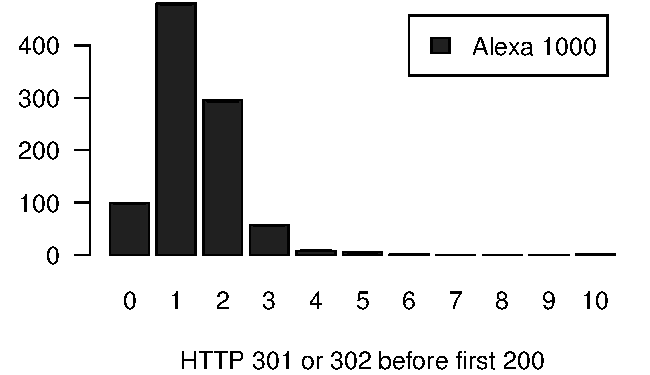
\includegraphics[width=.8\linewidth,keepaspectratio]{New_Plots/barplot_redirects_clean.pdf}
	\caption{New Measurements}
	\label{fig:new_bar_redirects}
	\par\medskip
	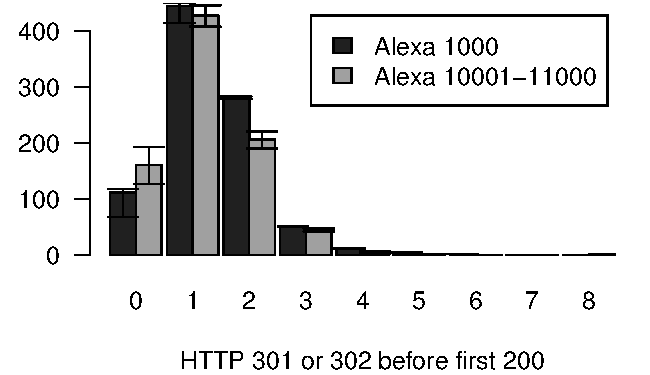
\includegraphics[width=.8\linewidth,keepaspectratio]{Original Plots/barplot_redirects.pdf}
	\caption{Original Measurements}
	\label{fig:orig_bar_redirects}
	\end{subfigure}%
	 \begin{subfigure}{0.5\textwidth}
	 \centering
	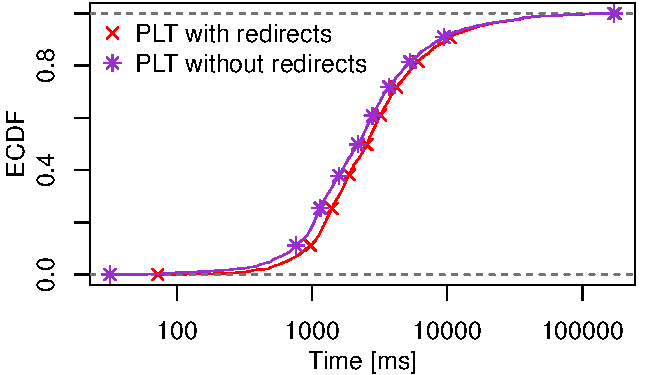
\includegraphics[width=.8\linewidth,keepaspectratio]{New_Plots/ecdf_loadtimes.pdf}
	\caption{New Measurements}
	\label{fig:new_plot_redirects}
	\par\medskip
	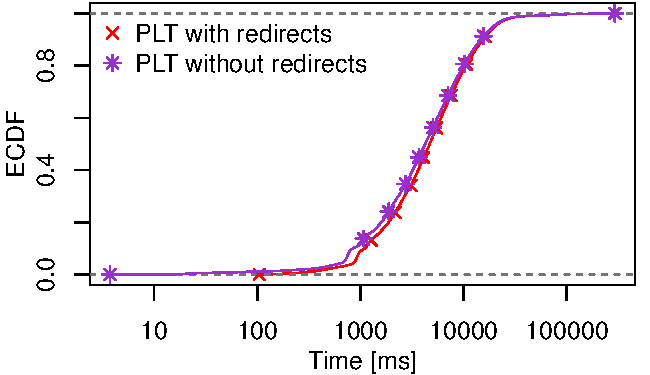
\includegraphics[width=.8\linewidth,keepaspectratio]{Original Plots/ecdf_loadtimes.pdf}
	\caption{Original Measurements}
	\label{fig:orig_plot_redirects}
	\end{subfigure}
\caption{Number of initial Redirects (Left) \& PLT with and without initial redirects (Right)}
\end{figure}

\end{frame}

\begin{frame}
    \frametitle{Results - Object Sizes}
\begin{figure}
 \centering
 \begin{subfigure}{0.5\textwidth}
 \centering
 	 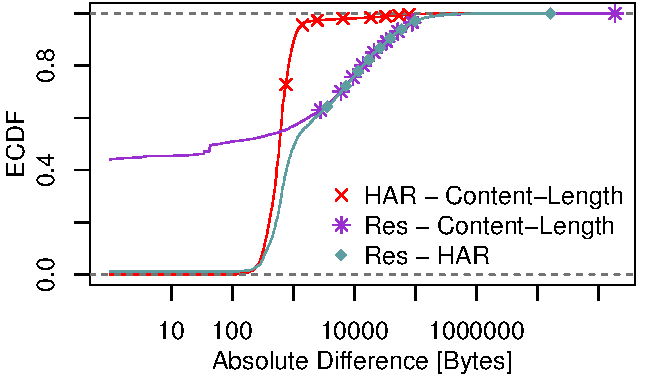
\includegraphics[width=\linewidth,keepaspectratio]{New_Plots/ecdf_diff_objectsizes.pdf}
	\caption{New Measurements}
	\label{fig:new_absolute_byte_index}
	\end{subfigure}%
	 \begin{subfigure}{0.5\textwidth}
	 \centering
	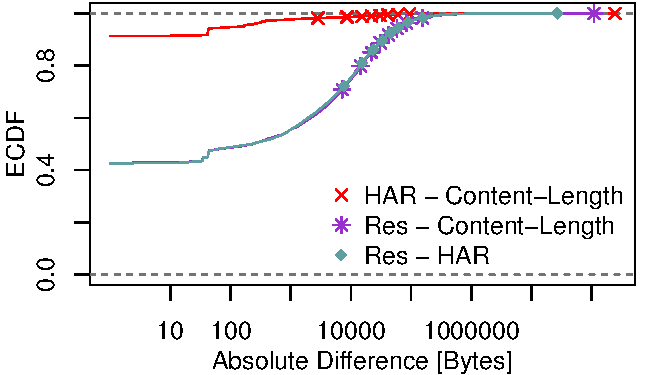
\includegraphics[width=.8\linewidth,keepaspectratio]{Firefox Plots/ecdf_diff_objectsizes.pdf}
	\caption{Original Measurements (Firefox Only)}
	\label{fig:orig_absolute_byte_index}
	\par\medskip
	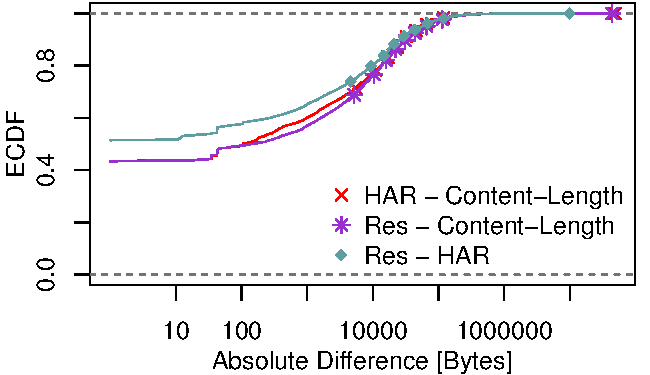
\includegraphics[width=.8\linewidth,keepaspectratio]{Chrome_Plots/ecdf_diff_objectsizes.pdf}
	\caption{Original Measurements (Chrome Only)}
	\label{fig:orig_chrome_absolute_byte_index}
	\end{subfigure}
\caption{Object sizes: differences due to metric for all objects}
\end{figure}

\end{frame}


\begin{frame}
    \frametitle{Results - Object Counts / Byte Index}
\begin{figure}
 \centering
 \begin{subfigure}{0.5\textwidth}
 \centering
 	 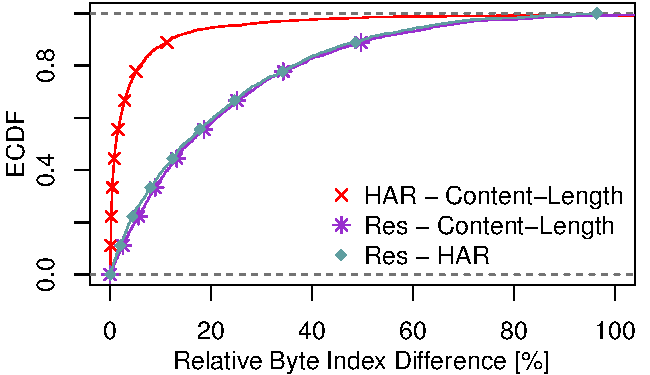
\includegraphics[width=\linewidth,keepaspectratio]{New_Plots/ecdf_rel_object_byte_index.pdf}
	\caption{New Measurements}
	\label{fig:new_relative_byte_index}

	\end{subfigure}%
	 \begin{subfigure}{0.5\textwidth}
	 \centering
	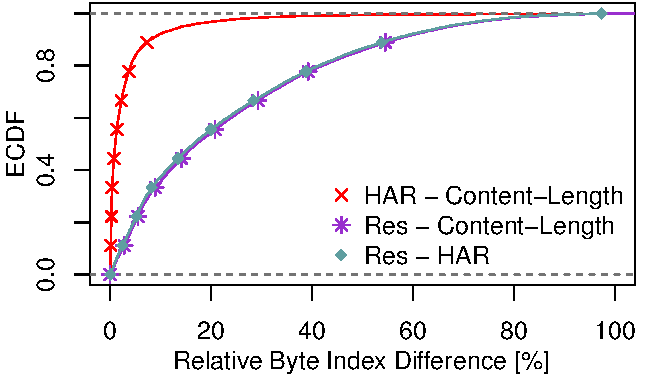
\includegraphics[width=.8\linewidth,keepaspectratio]{Firefox Plots/ecdf_rel_object_byte_index.pdf}
	\caption{Original Measurements (Firefox Only)}
	\label{fig:orig_firefox_relative_byte_index}
		\par\medskip
		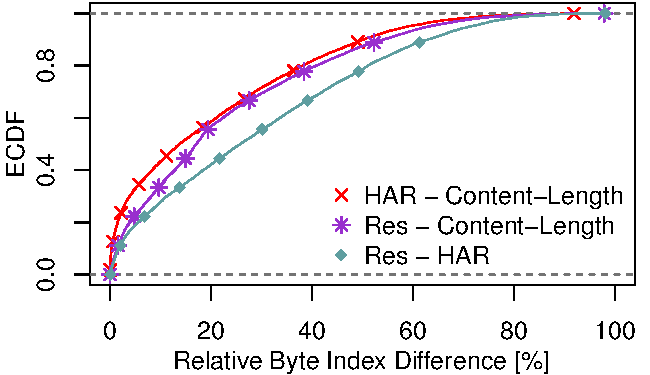
\includegraphics[width=.8\linewidth,keepaspectratio]{Chrome_Plots/ecdf_rel_object_byte_index.pdf}
	\caption{Original Measurements (Chrome Only)}
	\label{fig:orig_chrome_relative_byte_index}
	\end{subfigure}
\caption{Byte index: difference due to data source}
\end{figure}

\end{frame}
